Aquí pueden encontrarse gráficos adicionales sobre los métodos empleados
en este trabajo.

\subsubsection{Ley de Zipf}
\label{appendix-plots-zipf-law}

\begin{figure}[!htb]
    \centering
    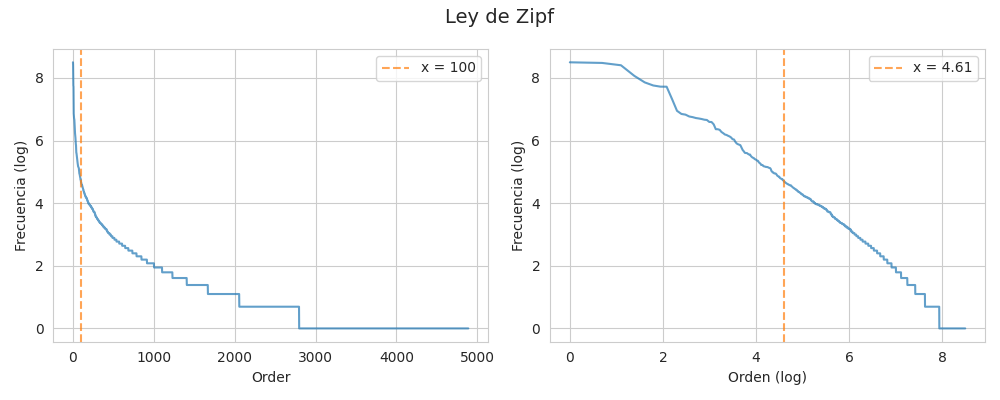
\includegraphics[scale=0.4]{../visualizations/ley_de_zipf.png}
    \caption{Contraste entre la frecuencia absoluta de cada palabra (en logaritmo)
    y el \textit{ranking} de esa palabra según su frecuencia. El gráfico de la
    derecha exhibe el orden natural de cada palabra y el de la izquierda, su logaritmo.
    En ambos casos, la línea punteada naranja indica el umbral
    para considerar \textit{stopword} a una palabra.}
    \label{fig-zipf-law}
\end{figure}
\FloatBarrier

\subsubsection{Selección de vectorizador}
\label{appendix-plots-vectorizers}

\begin{figure}[!htb]
    \centering
    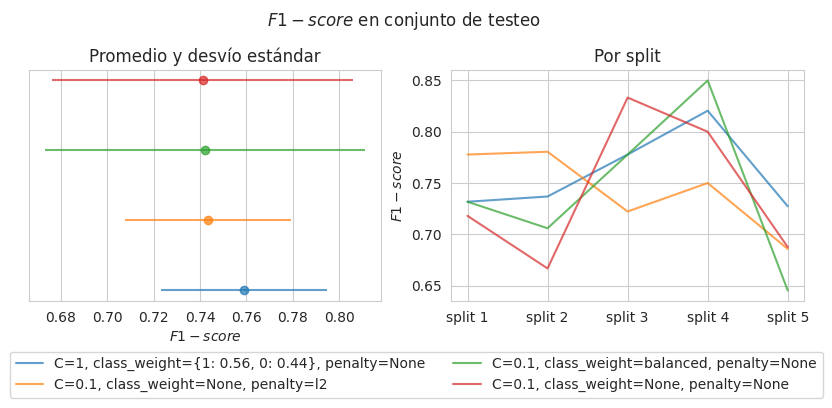
\includegraphics[scale=0.4]{../visualizations/features/f1_by_split.png}
    \caption{\textit{F1} por split de validación cruzada para el conjunto
    de entrenmiento y de testeo, para todos los vectorizadores en evaluación.}
    \label{fig-vectorizers-f1}
\end{figure}
\FloatBarrier

\begin{figure}[!htb]
    \centering
    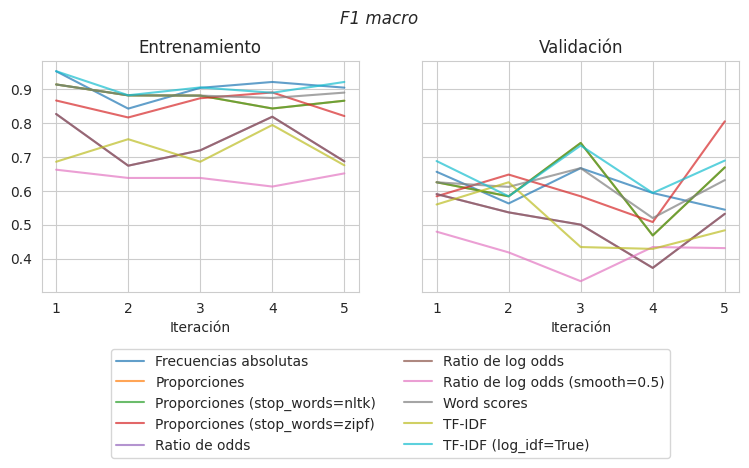
\includegraphics[scale=0.4]{../visualizations/features/f1_macro_by_split.png}
    \caption{\textit{F1-macro} por split de validación cruzada para el conjunto
    de entrenmiento y de testeo, para todos los vectorizadores en evaluación.}
    \label{fig-vectorizers-f1-macro}
\end{figure}
\FloatBarrier

\begin{figure}[!htb]
    \centering
    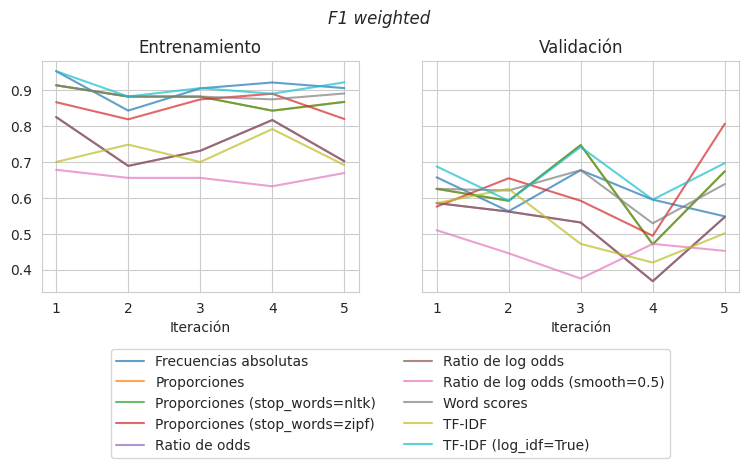
\includegraphics[scale=0.4]{../visualizations/features/f1_weighted_by_split.png}
    \caption{\textit{F1-weighted} o \textit{F1-pesado} por split de validación
    cruzada para el conjunto de entrenmiento y de testeo, para todos los
    vectorizadores en evaluación.}
    \label{fig-vectorizers-f1-weighted}
\end{figure}
\FloatBarrier

% cite title
%\usebibentry{monroe2008fightin}{title}